\documentclass[10pt]{article}
%% Specify the Express journal you are submitting to
%\usepackage[OME]{express}
\usepackage[OE]{express}
%\usepackage[BOE]{express}

\begin{document}

\title{Template and style guide for authors submitting to OSA Express Journals}

\author{Author One,\authormark{1} Author Two,\authormark{2,*} and Author Three\authormark{2,3}}

\address{\authormark{1}Peer Review, Publications Department, The Optical Society, 2010 Massachusetts Avenue NW, Washington, DC 20036, USA\\
\authormark{2}Publications Department, The Optical Society, 2010 Massachusetts Avenue NW, Washington, DC 20036, USA\\
\authormark{3}Currently with the Department of Electronic Journals, The Optical Society, 2010 Massachusetts Avenue NW, Washington, DC 20036, USA}

\email{\authormark{*}opex@osa.org} %% email address is required

% \homepage{http:...} %% author's URL, if desired

%%%%%%%%%%%%%%%%%%% abstract and OCIS codes %%%%%%%%%%%%%%%%
%% [use \begin{abstract*}...\end{abstract*} if exempt from copyright]

\begin{abstract}
Updated 14 July 2016. A template and instructions are provided for preparing \textit{Optics Express}, \textit{Biomedical Optics Express}, and \textit{Optical Materials Express} manuscripts in \LaTeX. A basic template is also available on \href{http://www.overleaf.com/docs?template=osa-opex-simple}{Overleaf}.
\end{abstract}

\ocis{(000.0000) General; (000.2700) General science.} % REPLACE WITH CORRECT OCIS CODES FOR YOUR ARTICLE, MINIMUM OF TWO; Avoid using the OCIS codes for “General” or “General science” whenever possible.
%For a complete list of OCIS codes, visit: https://www.osapublishing.org/oe/submit/ocis/

%%%%%%%%%%%%%%%%%%%%%%% References %%%%%%%%%%%%%%%%%%%%%%%%%
\begin{thebibliography}{99}
\bibitem{bib1}P. J. Harshman, T. K. Gustafson, and P. Kelley, ``Title of paper," J. Chem. Phys. {\bfseries 3}, (to be published).

\bibitem{gallo99} K. Gallo and G. Assanto, ``All-optical diode based on second-harmonic generation in an asymmetric waveguide,'' \josab {\bfseries 16}(2), 267--269 (1999).

\bibitem{Masters98a} B. R. Masters, ``Three-dimensional microscopic tomographic imagings of the cataract in a human lens in vivo,'' \opex {\bfseries 3}(9), 332--338 (1998).

\bibitem{Oron03} D. Yelin,  D. Oron,  S. Thiberge,  E. Moses, and Y. Silberberg, ``Multiphoton plasmon-resonance microscopy,'' \opex {\bfseries 11}(12), 1385--1391 (2003).

\bibitem{samplefig}
B.~N.~Behnken, G.~Karunasiri, D.~R.~Chamberlin, P.~R.~Robrish, and J.~Faist,
``Real-time imaging using a 2.8~THz quantum cascade laser and uncooled infrared microbolometer camera,'' \ol \textbf{33}(5), 440--442 (2008).

\end{thebibliography}

%%%%%%%%%%%%%%%%%%%%%%%%%%  body  %%%%%%%%%%%%%%%%%%%%%%%%%%
\section{Introduction}
Adherence to the specifications listed in this template is essential for efficient review and publication of submissions. Since OSA does not routinely perform copyediting and typesetting for this journal, use of the template is critical to providing a consistent appearance. Proper reference format is especially important (see Section \ref{sec:refs}).

\section{\texttt{express.sty} and required \LaTeX{} packages}
Page layout is set with the \texttt{geometry} package for US Letter paper. \texttt{express.sty} uses the following package files:

\begin{itemize}
\item \texttt{geometry} \ (page layout)
\item \texttt{color, graphicx} \ (replaces \texttt{graphics}; has preset options)
\item \texttt{mathptmx, courier, helvet} \ (Times, Courier, and Helvetica fonts)
\end{itemize}

The latest versions of these standard package files can be obtained at CTAN: the Comprehensive TeX Archive Network, \url{http://www.ctan.org}.

The command \verb+\usepackage{ae}+ can be invoked to revert font to Computer Modern, although we prefer to publish with Times (with \texttt{mathptmx.sty}) for consistency.

\section{Multiple corresponding authors}

There are two options for indicating multiple corresponding authorship, and they are formatted quite differently. The first format would be as follows, still using the asterisk to denote one of the authors:

\begin{verbatim}
\author{Author One\authormark{1,3} and Author Two\authormark{2,4}}

\address{\authormark{1}Peer Review, Publications Department,
Optical Society of America, 2010 Massachusetts Avenue NW,
Washington, DC 20036, USA\\
\authormark{2}Publications Department, Optical Society of America,
2010 Massachusetts Avenue NW, Washington, DC 20036, USA\\
\authormark{3}dmcdonold@osa.org}

\email{\authormark{*}opex@osa.org}
\end{verbatim}

This format will generate the following appearance:\\

\author{Author One\authormark{1,3} and Author Two\authormark{2,4}}

\address{\authormark{1}Peer Review, Publications Department,
Optical Society of America, 2010 Massachusetts Avenue NW,
Washington, DC 20036, USA\\
\authormark{2}Publications Department, Optical Society of America,
2010 Massachusetts Avenue NW, Washington, DC 20036, USA\\
\authormark{3}dmcdonold@osa.org}

\email{\authormark{*}opex@osa.org}
\medskip
The second format forgoes the asterisk and sets all email addresses equally within the affiliations. Please note that this format does not use the \verb+\email{}+ field at all.
\begin{verbatim}
\author{Author One\authormark{1,3} and Author Two\authormark{2,4}}

\address{\authormark{1}Peer Review, Publications Department,
Optical Society of America, 2010 Massachusetts Avenue NW,
Washington, DC 20036, USA\\
\authormark{2}Publications Department, Optical Society of America,
2010 Massachusetts Avenue NW, Washington, DC 20036, USA\\
\authormark{3}dmcdonold@osa.org\\
\authormark{4}opex.osa.org}
\end{verbatim}

This format will generate the following appearance:\\

\author{Author One\authormark{1,3} and Author Two\authormark{2,4}}

\address{\authormark{1}Peer Review, Publications Department,
Optical Society of America, 2010 Massachusetts Avenue NW, Washington, DC 20036, USA\\
\authormark{2}Publications Department, Optical Society of America, 2010 Massachusetts Avenue NW, Washington, DC 20036, USA\\
\authormark{3}dmcdonold@osa.org\\
\authormark{4}opex.osa.org}
\medskip
These are the preferred express journal formats for multiple corresponding authorship, and either may be used.

\section{Abstract}
The abstract should be limited to approximately 100 words. It should be an explicit summary of the paper that states the problem, the methods used, and the major results and conclusions. It also should contain the relevant key words that would allow it to be found in a cursory computerized search. If the work of another author is cited in the abstract, that citation should be written out without a number, [e.g., journal, volume, first page, and year (Opt. Express {\bfseries 22}, 1234 (2014))], and a separate citation should be included in the body of the text. The first reference cited in the main text must be [1]. Do not include numbers, bullets, or lists inside the abstract.

\section{Figures, tables, and supplemental materials}

\subsection{Figures and tables}

OSA express journals encourage authors to submit color and multimedia figures with their manuscripts. Figures and tables should be placed in the body of the manuscript.

\begin{figure}[ht!]
\centering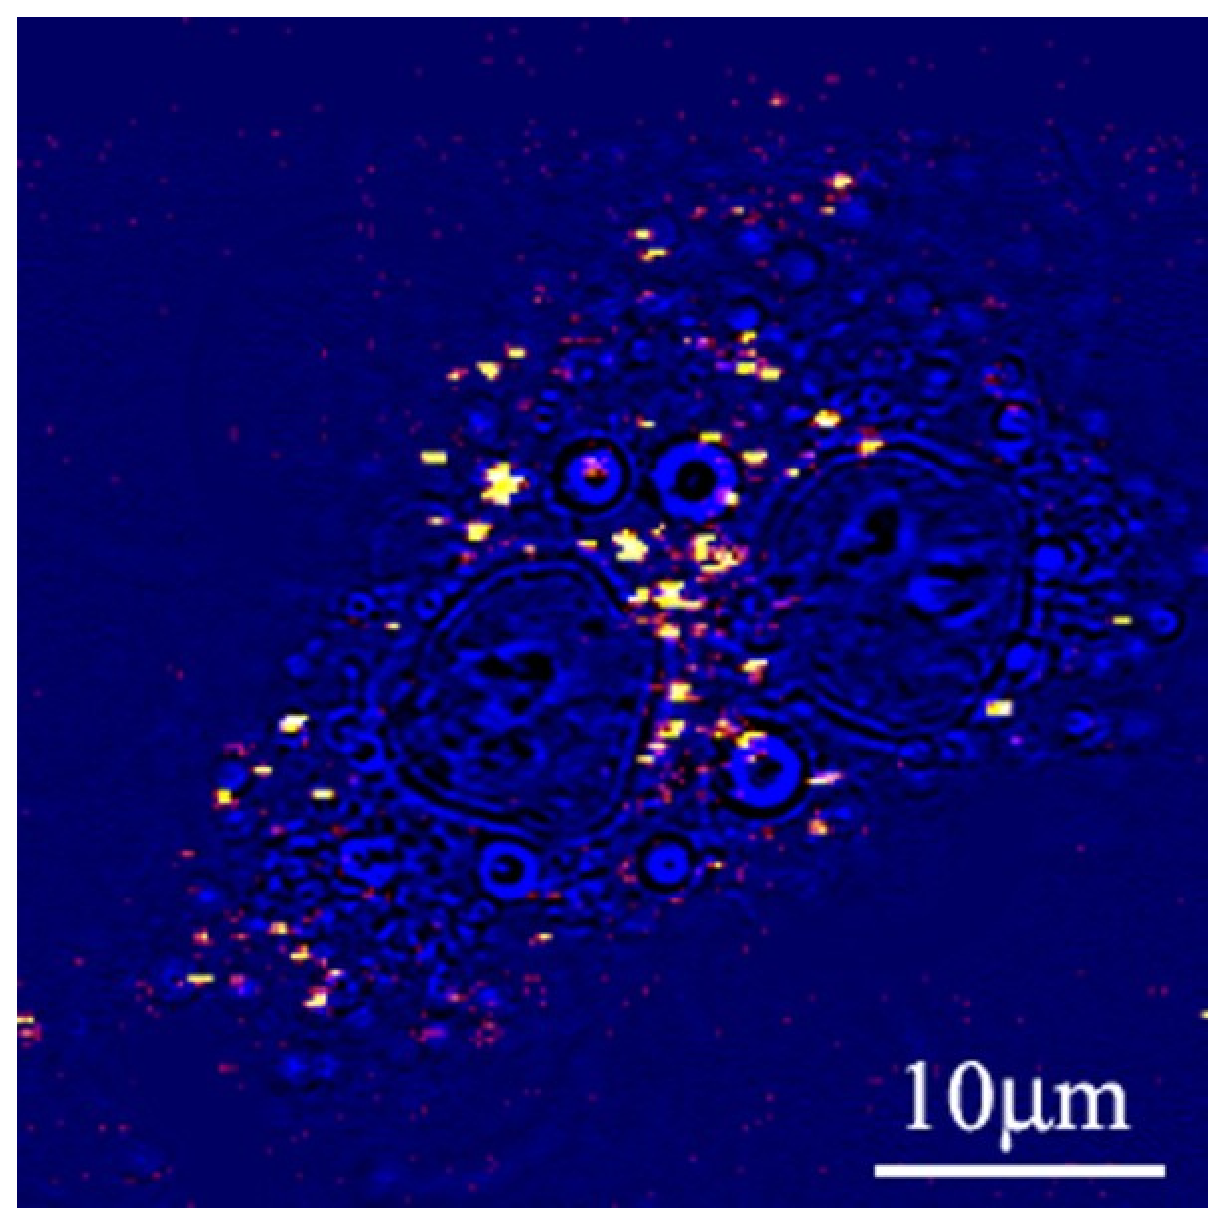
\includegraphics[width=7cm]{expressfig1}
\caption{Sample caption (Ref. \cite{Oron03}, Fig. 2).}
\end{figure}

\noindent Standard \LaTeX{} environments should be used to place tables and figures:
\begin{verbatim}
\begin{figure}[htbp]
\centering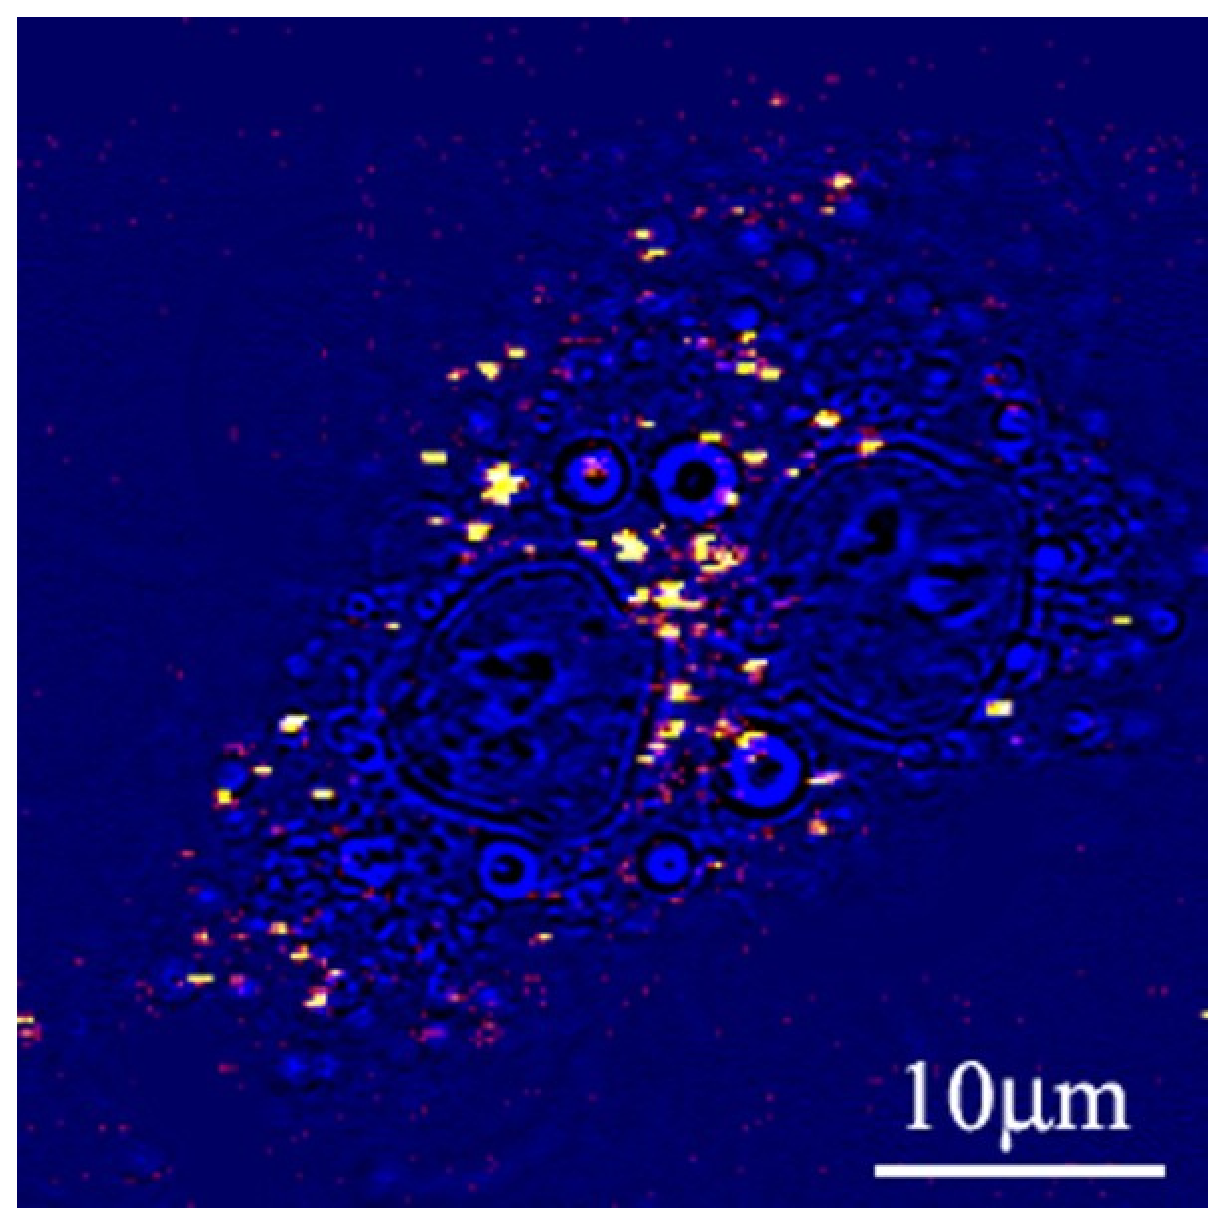
\includegraphics[width=7cm]{expressfig1}
\caption{Sample caption (Ref. \cite{Oron03}, Fig. 2).}
\end{figure}
\end{verbatim}

\subsection{Supplementary materials in OSA express journals}

Most OSA journals allow authors to include supplementary materials as integral parts of a manuscript. Such materials are subject to the same editorial standards and peer review procedures along with the rest of the paper and should be uploaded and described using OSA’s Prism manuscript system.

Authors can submit appropriate visualizations or small data files (see details below) for OSA to host. Large datasets and code or simulation files can be included but must be placed in an appropriate archival repository and cited as described here.

\begin{table}[ht!]
\centering
\caption{Supplementary Materials Supported in OSA Express Journals}
\begin{tabular}{|l|l|}
\hline
Visualization & 2D image, 3D image, video \\ \hline
Data File     & Small data file such as data underlying a plot in a figure \\ \hline
Dataset       & Dataset stored in an appropriate external repository \\ \hline
Code          & Code or simulation files stored in an appropriate external repository \\
\hline
\end{tabular}
\end{table}

Video visualizations (formerly media files) are the most commonly submitted type of supplementary materials for the express journals. They typically illustrate a synopsis of research results. They are integral and as such should be included only when they convey essential information beyond what can be presented within the article's PDF representation. Video visualizations should be uploaded upon submission and peer-reviewed along with the manuscript. Video files must use open compression standards for display on broadly available applications such as VLC or Windows Media Player. MOV, AVI, MPG, and MP4 video containers are accepted. The following video guidelines will help with the submission process:

\begin{itemize}
\item 15 MB is the recommended maximum video file size.
\item 720 x 480 pixels (width by height) is the recommended screen size.
\item If appropriate, insert a representative frame from the video in the manuscript as a figure.
\item Minimize file size by using an acceptable codec such as x264 or XviD. \href{https://handbrake.fr/}{HandBrake} is an open source tool for converting video to common codecs.
\item Video files must use open compression standards for display on broadly available applications such as VLC. 
\item Animations must be formatted into a standard video container.
\end{itemize}

Visualizations must be associated with a figure, table, or equation OR be referenced in the results section of the manuscript. Use the label ``Visualization" and the item number to identify the visualization. Please note that to create text color for supplementary materials links, use of the color.sty package and the command \verb|\textcolor{blue}{Visualization}| is preferred to using the command \verb|\url{Visualization}|.

\newpage

\begin{figure}[ht!]
\centering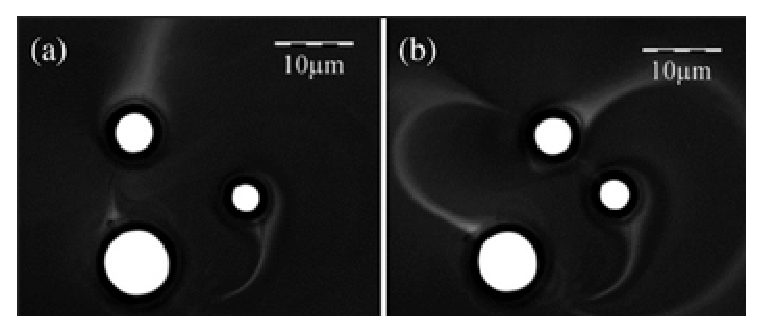
\includegraphics{expressfig2}
\caption{Three traps create three rings of magnetic nanoparticles. The rings interact with one another (see \textcolor{blue}{Visualization 3}). [From Masajada et al., Opt. Lett. \textbf{38}, 3910 (2013).]}
\end{figure}

\begin{verbatim}
\begin{figure}[h]
\centering\includegraphics{opexfig2}
\caption{Three traps create three rings of magnetic
nanoparticles. The rings interact with one another (see
\textcolor{blue}{Visualization 3}). [From Masajada
et al., Opt. Lett. \textbf{38}, 3910 (2013).]}
\end{figure}
\end{verbatim}

Please refer to the \href{http://www.osapublishing.org/submit/style/multimedia.cfm}{Author Guidelines for Supplementary Materials} for more detailed instructions on acceptable multimedia formats for audio and tabular data.


\section{Mathematical and scientific notation}

\subsection{Displayed equations} Displayed equations should be centered.
Equation numbers should appear at the right-hand margin, in
parentheses:
\begin{equation}
H = \frac{1}{2m}(p_x^2 + p_y^2) + \frac{1}{2} M{\Omega}^2
     (x^2 + y^2) + \omega (x p_y - y p_x).
\end{equation}

All equations should be numbered in the order in which they appear
and should be referenced  from within the main text as Eq. (1),
Eq. (2), and so on [or as inequality (1), etc., as appropriate].

\subsection{Inline math} To help with conversion, place all math in a proper math environment. For example, expression \mbox{$3\times 4 = 12$} should be set this way, \texttt{\$3$\backslash$times 4=12\$}, not this way, \texttt{3 \$$\backslash$times\$4=12}. Simple fractions for inline math
should use parentheses when necessary to avoid ambiguity, for
example, to distinguish between $1/(n-1)$ and $1/n-1$.  Exceptions
to this are the proper fractions such as $\frac{1}{2}$, which are
better left in this form. Summations and integrals that appear
within text such as $\frac{1}{2}{\sum }_{n=1}^{n=\infty} (n^2 -
2n)^{-1}$ should have limits placed to the right of the symbol to
reduce white space.

\subsection{General guidelines on notation} Notation must be
legible, clear, compact, and consistent with standard usage. In
general, acronyms should be defined at first use. Adherence to the
following guidelines will greatly assist the production process:

\paragraph*{\bfseries Radical signs.}
When possible, avoid oversized radical signs
by using the notation of a superscript $1/2$. For example, change
$\sqrt{(a + b)(a - c)}$ to $[(a + b)(a - c)]^{1/2}$.

\paragraph*{\bfseries Exponentials.} Avoid tiny superscripts of exponential $e$ (e.g.,
$e^{jkl})$ by using the alternative \verb+\exp+ notation,
$\exp(jkl)$.

\paragraph*{\bfseries Variables and vectors.}
Set single-letter variables in italics $(k)$. Set three-vectors in
boldface $(\mathbf{k})$. Functions, derivative ``d,''
abbreviations, and multiletter identifiers should be set in roman
(plain) type  ($\alpha \cos, \int\!\dots{d}x, k^{out}$).

\paragraph*{\bfseries Multiplication.}
In general, close up multiplied terms $(p_yp_x)$;
use $\times$ if multiplication sign is essential $(2 \times
10^{-2})$ or for continuation in displayed equations. Use raised dot only for scalar product $(\mathbf{k \cdot k})$.

\paragraph*{\bfseries Fences.}
For simple bracketing the usual order of parentheses and brackets
is $\{ \, [  \, (  \,  \{  \, [  \, (  \, |  \, )  \, ]  \, \} \,
)  \, ]  \, \}$.


\paragraph*{\bfseries Metric system.}
The metric system is used in OSA journals. If nonmetric units are
essential (e.g., for parts specifications), conversion should be
given at first mention:  ``. . . a $\frac{1}{4}$\,-in. bolt \mbox{(1 in.
= 2.54 cm).''}

\section*{Funding}
Please identify all appropriate funding sources by name and contract number. Funding information should be listed in a separate block preceding any acknowledgments.

List only the funding agencies and any associated grants or project numbers, as shown in the example below:\\
National Science Foundation (NSF) (1253236, 0868895, 1222301); Program 973 (2014AA014402); Natural National Science Foundation (NSFC) (123456).

OSA participates in \href{http://www.crossref.org/fundingdata/}{Crossref's Funding Data}, a service that provides a standard way to report funding sources for published scholarly research. To ensure consistency, please enter any funding agencies and contract numbers from the Funding section in Prism during submission or revisions.

\section*{Acknowledgments} Acknowledgments, if included, should appear at the end of the document. The section title should not follow the numbering scheme of the paper. Use the command \verb+\section*{Acknowledgments}+  to create a nonnumbered section heading. Please do not include any funding sources in the Acknowledgment section.

\section{References}
\label{sec:refs}
Proper formatting of references is extremely important, not only for consistent appearance but also for accurate electronic tagging. Please follow the guidelines provided below on formatting, callouts, and use of Bib\TeX.

\subsection{Formatting reference items}
Each source must have its own reference number. Footnotes (notes at the bottom of text pages) are not used in OSA journals. References require all author names, full titles, and inclusive pagination. Here are some examples of how to set the most common reference types:

\begin{description}
\item[Journal paper] \hfill\\
{\itshape Do not include web addresses in journal citations.}

C. van Trigt, ``Visual system-response functions and estimating reflectance,'' %\josaa
   J. Opt. Soc. Am. A {\bfseries 14}(4), 741--755 (1997).

S. Yerolatsitis, I. Gris-S\'anchez, and T. A. Birks,
``Adiabatically-tapered fiber mode multiplexers,'' Opt. Express {\bfseries 22}(1), 608--617 (2014).

\item[Journal paper identified by paper number] \hfill\\
{\itshape The paper number is sufficient. There is no need to give the number of pages.}

L. Rippe, B. Julsgaard, A. Walther, Y. Ying, and S. Kr\"oll,
``Experimental quantum-state tomography of a solid-state qubit,'' Phys. Rev. A {\bfseries 77}, 022307 (2008).

\item[Book] \hfill\\
T. Masters, {\itshape Practical Neural Network Recipes in C++} (Academic, 1993).

F. Ladouceur and J. D. Love, \textit{Silica-Based Buried Channel Waveguides and Devices} (Chapman \& Hall, 1995), Chap. 8.

\item[Article in a book] \hfill\\
D. F. Edwards, ``Silicon (Si),'' in {\itshape Handbook of Optical Constants of Solids,} E. D. Palik, ed. (Academic, 1985).

\item[Paper in a published conference proceedings] \hfill\\
R. E. Kalman, ``Algebraic aspects of the generalized inverse of a
rectangular matrix,'' in {\itshape Proceedings of Advanced Seminar on
Generalized Inverse and Applications,} M. Z. Nashed, ed. (Academic, 1976), pp. 111--124.

\item[Paper published in an OSA conference proceedings] \hfill\\
R. Craig and B. Gignac, ``High-power 980-nm pump lasers,'' in
{\itshape Optical Fiber Communication Conference}, Vol. 2 of 1996 OSA Technical Digest Series
(Optical Society of America, 1996), paper ThG1.

\item[Paper presented at a meeting/from an unpublished conference proceeding] \hfill\\
D. Steup and J. Weinzierl, ``Resonant THz-meshes,'' presented at the
Fourth International Workshop on THz Electronics,
Erlangen-Tennenlohe, Germany, 5--6 Sept. 1996.

\item[SPIE proceedings] \hfill\\
S. K. Griebel, M. Richardson, K. E. Devenport, and H. S. Hinton,
``Experimental performance of an ATM-based buffered hyperplane
CMOS-SEED smart pixel array,'' Proc. SPIE {\bfseries 3005}, 254--256 (1997).

{\itshape For later SPIE proceedings with a paper number, cite just the number and not any page information.}

S. Gu, F. Shao, G. Jiang, F. Li, and M. Yu,
``An objective visibility threshold measurement method for asymmetric stereoscopic images,''
Proc. SPIE {\bfseries 8205}, 820505 (2011).

\item[IEEE proceedings] \hfill\\
T. Darrel and K. Wohn, ``Pyramid based depth from focus,'' in
{\itshape Proceedings of IEEE Conference on Computer Vision and Pattern
Recognition} (IEEE, 1988), pp. 504--509.

\item[Paper accepted for publication] \hfill\\
D. Piao, ``Cancelation of coherent artifacts in optical coherence tomography imaging,'' Appl. Opt. (to be published).

D. W. Diehl and T. D. Visser,
"Phase singularities of the longitudinal field components in the focal region of a high-aperture optical system,"
J. Opt. Soc. Am. A, doc. ID 56789 (posted 11 November 2005, in press).

\item[Manuscript in preparation] \hfill\\
J. Q. Smith, Laboratory for Laser Energetics, University of Rochester, 250 East River Road, Rochester, New York 14623, USA, and K. Marshall are preparing a manuscript to be called ``Optical aspects in liquid crystals.''

\item[Personal communication] \hfill\\
T. Miller, Publications Department, Optical Society of
America, 2010 Massa\-chusetts Avenue, N.W., Washington, D.C.,
20036 (personal communication, 2010).

\item[Internet links] \hfill\\
Extreme Networks white paper, ``Virtual metropolitan area networks,'' (Extreme Networks, 2001), \texttt{http://www.extremenetworks.com/technology/
whitepapers/vMAN.asp}.

A. G. Ramm, ``Invisible obstacles,'' \texttt{http://www.arxiv.org/abs/math-ph
/0608034}.

\end{description}

The commands \verb+\begin{thebibliography}{}+ and \verb+\end{thebibliography}+ format the section according to standard style, showing the title {\bfseries References and links}.  Use the \verb+\bibitem{label}+ command to start each reference.

\subsection{Formatting reference citations}
References should be numbered consecutively in the order in which they are referenced in the body of the paper. Set reference callouts with standard \verb+\cite{}+ command or set manually inside square brackets [1].

To reference multiple articles at once, simply use the cite command with a comma separating the reference labels, e.g. \verb+\cite{gallo99,Masters98a,Oron03}+, produces \cite{gallo99,Masters98a,Oron03}. Using the \texttt{cite.sty} package will make these citations appear like so: [2--4].

\subsection{Bib\TeX}
\label{sec:bibtex}
Bib\TeX{} may be used to create a file containing the references, whose contents (i.e., contents of \texttt{.bbl} file) can then be pasted into the bibliography section of the \texttt{.tex} file. A new Bib\TeX{} style file, \texttt{osajnl.bst}, is provided.

To assist authors with journal abbreviations in references, standard abbreviations for some commonly cited journals have been included as macros within opex3.sty.  The abbreviations are shown in Table 2 below.

\begin{table}[htbp]
\centering\caption{Standard abbreviations
 for commonly cited journals.}
\begin{tabular}{lp{1.7in}|lp{1.7in}}
\hline
Macro        & Abbreviation                & Macro        & Abbreviation          \\ \hline
\verb+\ao+   & Appl.\  Opt.\               & \verb+\jpp+  & J. Phys.              \\
\verb+\aop+  & Adv. Opt. Photon.           & \verb+\nat+  & Nature                \\
\verb+\ap+   & Appl.\  Phys.\              & \verb+\oc+   & Opt.\ Commun.\        \\
\verb+\apl+  & Appl.\ Phys.\ Lett.\        & \verb+\opex+ & Opt.\ Express         \\
\verb+\apj+  & Astrophys.\ J.\             & \verb+\ol+   & Opt.\ Lett.\          \\
\verb+\bell+ & Bell Syst.\ Tech.\ J.\      & \verb+\ome+  & Opt.\ Mater.\ Express \\
\verb+\boe+  & Biomed.\ Opt.\ Express      & \verb+\opn+  & Opt.\ Photon.\ News   \\
\verb+\jqe+ & IEEE J.\ Quantum Electron.\  & \verb+\pl+   & Phys.\ Lett.\         \\
\verb+\assp+ & IEEE Trans.\ Acoust.\ Speech Signal Process.\  & \verb+\pr+ & Photon.\ Res.\ \\
\verb+\aprop+ & IEEE Trans.\  Antennas Propag.\    & \verb+\pra+ & Phys.\ Rev.\ A   \\
\verb+\mtt+ & IEEE Trans.\ Microwave Theory Tech.\ & \verb+\prb+ & Phys.\ Rev.\ B   \\
\verb+\iovs+ & Invest.\ Ophthalmol.\ Vis.\ Sci.\    & \verb+\prc+ & Phys.\ Rev.\ C   \\
\verb+\jcp+ & J.\ Chem.\ Phys.\            & \verb+\prd+ & Phys.\ Rev.\ D   \\
\verb+\jmo+ & J.\ Mod.\ Opt.\              & \verb+\pre+ & Phys.\ Rev.\ E   \\
\verb+\jocn+ & J.\ Opt.\ Commun.\ Netw.\   & \verb+\prl+ & Phys.\ Rev.\ Lett.\    \\
\verb+\jon+ & J.\ Opt.\ Netw.\             & \verb+\rmp+ & Rev.\ Mod.\ Phys.\    \\
\verb+\josa+ & J.\ Opt.\ Soc.\ Am.\        & \verb+\pspie+ & Proc.\ Soc.\ Photo-Opt.\ Instrum.\ Eng.\   \\
\verb+\josaa+ & J.\ Opt.\ Soc.\ Am.\ A     & \verb+\sjqe+ & Sov.\ J.\ Quantum Electron.\   \\
\verb+\josab+ & J.\ Opt.\ Soc.\ Am.\ B     & \verb+\vr+ & Vision Res.\   \\ \hline
\end{tabular}
\end{table}


\section{Conclusion}
After proofreading the manuscript, compress your .TEX manuscript file and all figures (which should be in EPS format, or PDF format if you are using PDF-\LaTeX) in a ZIP, TAR or TAR-GZIP package. Prism, OSA’s article tracking system, will process in \LaTeX mode by default but will use PDF-\LaTeX if PDF figure files are detected. Note: TAR or TAR-GZIP is no longer required. All files must be referenced at the root level (e.g., file \texttt{figure-1.eps}, not \texttt{/myfigs/figure-1.eps}). If there is video or other supplementary materials, the associated files should be uploaded separately.

\end{document}
